% Options for packages loaded elsewhere
\PassOptionsToPackage{unicode}{hyperref}
\PassOptionsToPackage{hyphens}{url}
\PassOptionsToPackage{dvipsnames,svgnames*,x11names*}{xcolor}
%
\documentclass[
  8pt,
  ignorenonframetext,
  dvipsnames]{beamer}
\usepackage{pgfpages}
\setbeamertemplate{caption}[numbered]
\setbeamertemplate{caption label separator}{: }
\setbeamercolor{caption name}{fg=normal text.fg}
\beamertemplatenavigationsymbolsempty
% Prevent slide breaks in the middle of a paragraph
\widowpenalties 1 10000
\raggedbottom
\setbeamertemplate{part page}{
  \centering
  \begin{beamercolorbox}[sep=16pt,center]{part title}
    \usebeamerfont{part title}\insertpart\par
  \end{beamercolorbox}
}
\setbeamertemplate{section page}{
  \centering
  \begin{beamercolorbox}[sep=12pt,center]{part title}
    \usebeamerfont{section title}\insertsection\par
  \end{beamercolorbox}
}
\setbeamertemplate{subsection page}{
  \centering
  \begin{beamercolorbox}[sep=8pt,center]{part title}
    \usebeamerfont{subsection title}\insertsubsection\par
  \end{beamercolorbox}
}
\AtBeginPart{
  \frame{\partpage}
}
\AtBeginSection{
  \ifbibliography
  \else
    \frame{\sectionpage}
  \fi
}
\AtBeginSubsection{
  \frame{\subsectionpage}
}
\usepackage{lmodern}
\usepackage{amssymb,amsmath}
\usepackage{ifxetex,ifluatex}
\ifnum 0\ifxetex 1\fi\ifluatex 1\fi=0 % if pdftex
  \usepackage[T1]{fontenc}
  \usepackage[utf8]{inputenc}
  \usepackage{textcomp} % provide euro and other symbols
\else % if luatex or xetex
  \usepackage{unicode-math}
  \defaultfontfeatures{Scale=MatchLowercase}
  \defaultfontfeatures[\rmfamily]{Ligatures=TeX,Scale=1}
\fi
% Use upquote if available, for straight quotes in verbatim environments
\IfFileExists{upquote.sty}{\usepackage{upquote}}{}
\IfFileExists{microtype.sty}{% use microtype if available
  \usepackage[]{microtype}
  \UseMicrotypeSet[protrusion]{basicmath} % disable protrusion for tt fonts
}{}
\makeatletter
\@ifundefined{KOMAClassName}{% if non-KOMA class
  \IfFileExists{parskip.sty}{%
    \usepackage{parskip}
  }{% else
    \setlength{\parindent}{0pt}
    \setlength{\parskip}{6pt plus 2pt minus 1pt}}
}{% if KOMA class
  \KOMAoptions{parskip=half}}
\makeatother
\usepackage{xcolor}
\IfFileExists{xurl.sty}{\usepackage{xurl}}{} % add URL line breaks if available
\IfFileExists{bookmark.sty}{\usepackage{bookmark}}{\usepackage{hyperref}}
\hypersetup{
  pdftitle={Introduction to Multivariate Regression \& Econometrics},
  pdfauthor={Lecture 9},
  colorlinks=true,
  linkcolor=Maroon,
  filecolor=Maroon,
  citecolor=Blue,
  urlcolor=blue,
  pdfcreator={LaTeX via pandoc}}
\urlstyle{same} % disable monospaced font for URLs
\newif\ifbibliography
\usepackage{graphicx,grffile}
\makeatletter
\def\maxwidth{\ifdim\Gin@nat@width>\linewidth\linewidth\else\Gin@nat@width\fi}
\def\maxheight{\ifdim\Gin@nat@height>\textheight\textheight\else\Gin@nat@height\fi}
\makeatother
% Scale images if necessary, so that they will not overflow the page
% margins by default, and it is still possible to overwrite the defaults
% using explicit options in \includegraphics[width, height, ...]{}
\setkeys{Gin}{width=\maxwidth,height=\maxheight,keepaspectratio}
% Set default figure placement to htbp
\makeatletter
\def\fps@figure{htbp}
\makeatother
\setlength{\emergencystretch}{3em} % prevent overfull lines
\providecommand{\tightlist}{%
  \setlength{\itemsep}{0pt}\setlength{\parskip}{0pt}}
\setcounter{secnumdepth}{-\maxdimen} % remove section numbering

%packages
\usepackage{graphicx}
\usepackage{rotating}
\usepackage{hyperref}

\usepackage{tikz} % used for text highlighting, amongst others
\usepackage{comment}

%title slide stuff
%\institute{Department of Education}
%\title{Managing and Manipulating Data Using R}

%
\setbeamertemplate{navigation symbols}{} % get rid of navigation icons:
\setbeamertemplate{footline}[page number]

%\setbeamertemplate{frametitle}{\thesection \hspace{0.2cm} \insertframetitle}
\setbeamertemplate{section in toc}[sections numbered]
%\setbeamertemplate{subsection in toc}[subsections numbered]
\setbeamertemplate{subsection in toc}{%
  \leavevmode\leftskip=3.2em\color{gray}\rlap{\hskip-2em\inserttocsectionnumber.\inserttocsubsectionnumber}\inserttocsubsection\par
}

%define colors
%\definecolor{uva_orange}{RGB}{216,141,42} % UVa orange (Rotunda orange)
\definecolor{mygray}{rgb}{0.95, 0.95, 0.95} % for highlighted text
	% grey is equal parts red, green, blue. higher values >> lighter grey
	%\definecolor{lightgraybo}{rgb}{0.83, 0.83, 0.83}

% new commands

%highlight text with very light grey
\newcommand*{\hlg}[1]{%
	\tikz[baseline=(X.base)] \node[rectangle, fill=mygray] (X) {#1};%
}
%, inner sep=0.3mm
%highlight text with very light grey and use font associated with code
\newcommand*{\hlgc}[1]{\texttt{\hlg{#1}}}

%modifying back ticks to add grey background
\let\OldTexttt\texttt
\renewcommand{\texttt}[1]{\OldTexttt{\hlg{#1}}}


\begin{comment}

% Font
\usepackage[defaultfam,light,tabular,lining]{montserrat}
\usepackage[T1]{fontenc}
\renewcommand*\oldstylenums[1]{{\fontfamily{Montserrat-TOsF}\selectfont #1}}

% Change color of boldface text to darkgray
\renewcommand{\textbf}[1]{{\color{darkgray}\bfseries\fontfamily{Montserrat-TOsF}#1}}

% Bullet points
\setbeamertemplate{itemize item}{\color{BlueViolet}$\circ$}
\setbeamertemplate{itemize subitem}{\color{BrickRed}$\triangleright$}
\setbeamertemplate{itemize subsubitem}{$-$}

% Reduce space before lists
%\addtobeamertemplate{itemize/enumerate body begin}{}{\vspace*{-8pt}}

\let\olditem\item
\renewcommand{\item}{%
  \olditem\vspace{4pt}
}

% decreasing space before and after level-2 bullet block
%\addtobeamertemplate{itemize/enumerate subbody begin}{}{\vspace*{-3pt}}
%\addtobeamertemplate{itemize/enumerate subbody end}{}{\vspace*{-3pt}}

% decreasing space before and after level-3 bullet block
%\addtobeamertemplate{itemize/enumerate subsubbody begin}{}{\vspace*{-2pt}}
%\addtobeamertemplate{itemize/enumerate subsubbody end}{}{\vspace*{-2pt}}

%Section numbering
\setbeamertemplate{section page}{%
    \begingroup
        \begin{beamercolorbox}[sep=10pt,center,rounded=true,shadow=true]{section title}
        \usebeamerfont{section title}\thesection~\insertsection\par
        \end{beamercolorbox}
    \endgroup
}

\setbeamertemplate{subsection page}{%
    \begingroup
        \begin{beamercolorbox}[sep=6pt,center,rounded=true,shadow=true]{subsection title}
        \usebeamerfont{subsection title}\thesection.\thesubsection~\insertsubsection\par
        \end{beamercolorbox}
    \endgroup
}

\end{comment}

\title{Introduction to Multivariate Regression \& Econometrics}
\subtitle{HED 612}
\author{Lecture 9}
\date{}

\begin{document}
\frame{\titlepage}

\begin{frame}
  \tableofcontents[hideallsubsections]
\end{frame}
\begin{frame}{Where are going\ldots{}}
\protect\hypertarget{where-are-going}{}

\textbf{Today:}

\begin{itemize}
\tightlist
\item
  Bias and Efficiency
\item
  Introduction to Multivariate regression

  \begin{itemize}
  \tightlist
  \item
    OLS Assumption 1 \& omitted variable bias
  \end{itemize}
\item
  Reading:

  \begin{itemize}
  \tightlist
  \item
    NONE
  \end{itemize}
\item
  Homework:

  \begin{itemize}
  \tightlist
  \item
    Homework Assignment \#9 posted on D2L
  \end{itemize}
\end{itemize}

\textbf{Next Week}

\begin{itemize}
\tightlist
\item
  Multivariate regression cont.
\item
  Reading:

  \begin{itemize}
  \tightlist
  \item
    Empirical manuscripts
  \end{itemize}
\end{itemize}

\textbf{Following week}

\begin{itemize}
\tightlist
\item
  Read empirical quantitative work
\end{itemize}

\end{frame}

\hypertarget{bias-and-efficiency}{%
\section{Bias and Efficiency}\label{bias-and-efficiency}}

\begin{frame}{Efficiency, also called ``precision''}
\protect\hypertarget{efficiency-also-called-precision}{}

\begin{itemize}
\tightlist
\item
  Desirable properties of our point estimates (e.g.~\(\hat{\beta}\) or
  \(\bar{Y}\))

  \begin{itemize}
  \tightlist
  \item
    Efficient
  \item
    Unbiased
  \end{itemize}
\item
  \textbf{Efficiency}

  \begin{itemize}
  \tightlist
  \item
    Definition: how close your point estimate(s) is to the population
    parameter
  \item
    Standard Error: on average, how far away is a point estimate from
    one random sample from the value of the population parameter
  \item
    \emph{Therefore}, an efficient point estimate is one with a low
    standard error (in other words, the sampling distribution of
    \(\beta_1\) has low variance or is ``tight'' around the population
    parameter)
  \end{itemize}
\end{itemize}

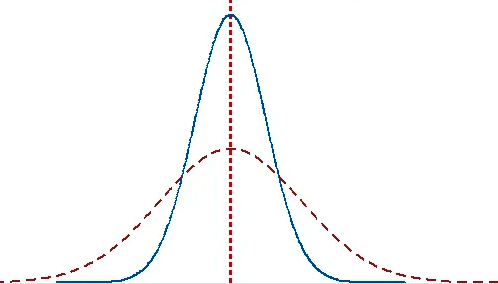
\includegraphics{precision.png}

\end{frame}

\begin{frame}{Bias}
\protect\hypertarget{bias}{}

\begin{itemize}
\tightlist
\item
  \textbf{Bias}: consistently overestimates or underestimates population
  parameter in repeated random samples

  \begin{itemize}
  \tightlist
  \item
    There are many different types of bias!
  \end{itemize}
\item
  \emph{Sampling Bias}:

  \begin{itemize}
  \tightlist
  \item
    Estimate of population parameter is biased because you fail to take
    a random sample
  \item
    Example: goal is to estimate high school graduation rate; take a
    random sample of 10th graders and see if they graduate within three
    years.
  \end{itemize}
\item
  \emph{Omitted variable bias}:

  \begin{itemize}
  \tightlist
  \item
    Bias in estimate of \(\beta_1\) due to omitting necessary
    ``control'' variables in your regression model
  \end{itemize}
\end{itemize}

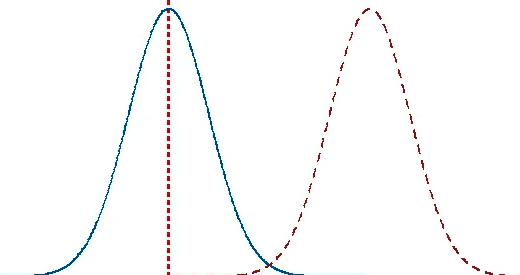
\includegraphics{bias.png}

\end{frame}

\begin{frame}{Bias and Efficiency (or ``Precision'')}
\protect\hypertarget{bias-and-efficiency-or-precision}{}

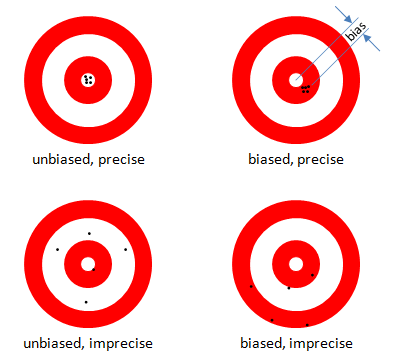
\includegraphics{bias_efficiency.png}

\end{frame}

\hypertarget{ols-assumption-1}{%
\section{OLS Assumption 1}\label{ols-assumption-1}}

\begin{frame}{Prior to assumptions: define causal effect}
\protect\hypertarget{prior-to-assumptions-define-causal-effect}{}

\begin{itemize}
\tightlist
\item
  Asking causal inference research questions

  \begin{itemize}
  \tightlist
  \item
    ``What is the effect of X on Y''
  \item
    Goal: to estimate the ``causal effect'' of X on Y
  \end{itemize}
\end{itemize}

\medskip

\begin{itemize}
\tightlist
\item
  What is a ``causal effect''?

  \begin{itemize}
  \tightlist
  \item
    Stock and Watson define it as ``what would happen in a randomized
    experiment''
  \item
    Causal effect is the average effect of being in the ``treatment''
    group as opposed to the ``control'' group on the value of Y if
    people were randomly assigned to groups
  \end{itemize}
\end{itemize}

\medskip

\begin{itemize}
\tightlist
\item
  How do you know if you are asking a causal inference research
  question?

  \begin{itemize}
  \tightlist
  \item
    As yourself, what is the relevant randomized experiment?
  \item
    That is, how would your question be designed as a randomized
    experiment?
  \end{itemize}
\end{itemize}

\end{frame}

\begin{frame}{Today's example \& defining causal effect}
\protect\hypertarget{todays-example-defining-causal-effect}{}

\begin{itemize}
\tightlist
\item
  RQ: What is the effect of federal financial aid on students' access to
  college (Cellini, 2008)?

  \begin{itemize}
  \tightlist
  \item
    Is this a causal inference research question?
  \item
    What is the relevant experiment?
  \item
    Are students randomly assigned to receive federal financial aid?
  \end{itemize}
\item
  Experimental data vs.~Observational data

  \begin{itemize}
  \tightlist
  \item
    Experimental data: people randomly assigned to ``treatment''
    vs.~``control'' group
  \end{itemize}
\item
  Cellini (2008): Multivariate regression can be used to deal with the
  problem that the ``treatment'' (in this case receiving federal
  financial aid) wasn't randomized in order to assess the effect of X on
  Y (receiving financial aid on college access).
\item
  We do our best to recreate experimental conditions for observational
  data by minimizing omitted variable bias (more on this later)!
\end{itemize}

\end{frame}

\begin{frame}{OLS Assumption 1 (mathematically)}
\protect\hypertarget{ols-assumption-1-mathematically}{}

\begin{itemize}
\tightlist
\item
  Population linear regression model

  \begin{itemize}
  \tightlist
  \item
    \(Y_i = \beta_0 + \beta_1 X_i+ u_i\)
  \item
    Y= years of schooling (12+ = attended college), X= 0/1 received
    financial aid, \(u_i\) = all other variables that affect Y but were
    not included in the model
  \end{itemize}
\item
  OLS Assumption 1 (in words)

  \begin{itemize}
  \tightlist
  \item
    the independent variable \(X_i\) is unrelated to the ``other
    variables'' not included in the model, \(u_i\)
  \end{itemize}
\item
  OLS Assumption 1 (mathematically)

  \begin{itemize}
  \tightlist
  \item
    \(E(u_i|X_i)=0\); the expected value of \(u_i\), given any value of
    \(X_i\), equals zero
  \item
    In other words:

    \begin{itemize}
    \tightlist
    \item
      Pretend that \(u_i\) consists of only one variable
    \item
      OLS assumption 1 states that the mean value of the omitted
      variable is equal to zero no matter the value of variable \(X_i\)
    \end{itemize}
  \end{itemize}
\end{itemize}

\end{frame}

\begin{frame}{OLS Assumption 1}
\protect\hypertarget{ols-assumption-1-1}{}

\begin{itemize}
\tightlist
\item
  OLS Assumption 1: \(E(u_i|X_i)=0\)
\item
  \textbf{Cellini 2008}: Assumption is \emph{always} satisfied in random
  assignment experiment

  \begin{itemize}
  \tightlist
  \item
    Effect of financial aid (X) on college access
  \item
    X=0 (did not receive financial aid); X=1 (received financial aid)
  \item
    We randomly assign students to receive versus not receive financial
    aid
  \item
    Other factors \(u_i\) (e.g., academic achievement, socioeconomic
    status) are \emph{by construction} unrelated to values of X because
    we randomly assigned students to X=1 or X=0
  \end{itemize}
\item
  \textbf{Cellini 2008}: in observational studies (like analyzing what
  is the effect of financial aid on student access to college), this
  assumption is usually violated!

  \begin{itemize}
  \tightlist
  \item
    For example, Receiving financial aid (X) is likely correlated with
    omitted variables, \(u_i\) that have an effect on Y (e.g., academic
    achievement, socioeconomic status)
  \end{itemize}
\end{itemize}

\end{frame}

\begin{frame}{OLS Assumption 1 in practice}
\protect\hypertarget{ols-assumption-1-in-practice}{}

\begin{itemize}
\tightlist
\item
  Population linear regression model

  \begin{itemize}
  \tightlist
  \item
    \(Y_i = \beta_0 + \beta_1 X_i+ u_i\)
  \item
    Y= years of schooling (12+ = attended college), X= 0/1 received
    financial aid, \(u_i\) = all other variables that affect Y but were
    not included in the model
  \end{itemize}
\item
  OLS Assumption 1 (in words)

  \begin{itemize}
  \tightlist
  \item
    the independent variable \(X_i\) is unrelated to the ``other
    variables'' not included in the model, \(u_i\)
  \end{itemize}
\item
  In Practice:

  \begin{itemize}
  \tightlist
  \item
    Are there any variables that are not in your model that\ldots{}
  \item
    \textbf{(1) Affect Y and (2) have a relationship (e.g.~correlated)
    with X}?
  \item
    If so, OLS Assumption 1 is violated
  \end{itemize}
\item
  Can you think of another omitted variable that violates OLS Assumption
  1 for this RQ?
\end{itemize}

\end{frame}

\begin{frame}{``No relationship'' vs ``No correlation''}
\protect\hypertarget{no-relationship-vs-no-correlation}{}

\begin{itemize}
\tightlist
\item
  Note: ``no relationship'' vs ``no correlation''

  \begin{itemize}
  \tightlist
  \item
    \(E(u_i|X_i)=0\) implies that \(u_i\) and \(X_i\) have no
    relationship (includes linear and non-linear)
  \item
    \(Corr(u_i|X_i)=0\) implies that \(u_i\) and \(X_i\) have no
    \emph{linear relationship}

    \begin{itemize}
    \tightlist
    \item
      e.g., Pearson's R correlation coefficient
    \end{itemize}
  \end{itemize}
\item
  So correlation might be zero, but \(E(u_i|X_i) \ne 0\) due to the
  existence of a non-linear relationship
\end{itemize}

\end{frame}

\hypertarget{omitted-variable-bias}{%
\section{Omitted Variable Bias}\label{omitted-variable-bias}}

\begin{frame}{Introduction to Omitted Variable Bias}
\protect\hypertarget{introduction-to-omitted-variable-bias}{}

\begin{itemize}
\tightlist
\item
  \(Y_i = \beta_0 + \beta_1X_i + u_i\); Y=test score; X=class size

  \begin{itemize}
  \tightlist
  \item
    We want to know the \emph{causal effect} of X on Y
  \end{itemize}
\end{itemize}

\medskip

\begin{itemize}
\tightlist
\item
  Bias (general): when \(\hat{\beta_1}\) consistently underestimates
  \(\beta_1\) or overestimates \(\beta_1\)
\end{itemize}

\medskip

\begin{itemize}
\tightlist
\item
  \textbf{Omitted Variable Bias}: bias in \(\hat{\beta_1}\) due to
  variables being omitted from the model
\end{itemize}

\medskip

\begin{itemize}
\tightlist
\item
  \textbf{For omitted variable bias to occur, the omitted variable ``Z''
  must satisfy two conditions}:

  \begin{itemize}
  \item
    \begin{enumerate}
    [(1)]
    \tightlist
    \item
      Z affects value of Y (i.e.~Z is part of \(u_i\))
    \end{enumerate}
  \item
    \begin{enumerate}
    [(1)]
    \setcounter{enumi}{1}
    \tightlist
    \item
      \emph{and} Z has a relationship with \(X\)
    \end{enumerate}
  \end{itemize}
\end{itemize}

\end{frame}

\begin{frame}{Omitted Variable Bias Example}
\protect\hypertarget{omitted-variable-bias-example}{}

\begin{itemize}
\tightlist
\item
  \(Y_i = \beta_0 + \beta_1X_i + u_i\)

  \begin{itemize}
  \tightlist
  \item
    Y= average class reading test score
  \item
    X= class size
  \item
    Z= \% of ELL students (omitted from model)
  \end{itemize}
\item
  For omitted variable bias to occur, the omitted variable ``Z'' must
  satisfy two conditions:

  \begin{itemize}
  \item
    \begin{enumerate}
    [(1)]
    \tightlist
    \item
      Z affects value of Y (i.e.~Z is part of \(u_i\));
    \end{enumerate}
  \item
    \begin{enumerate}
    [(1)]
    \setcounter{enumi}{1}
    \tightlist
    \item
      \textbf{and} Z has a relationship with \(X\)
    \end{enumerate}
  \end{itemize}
\item
  How does \% of ELL students satisfy criteria of omitted variable bias?

  \begin{itemize}
  \item
    \begin{enumerate}
    [(1)]
    \tightlist
    \item
      \% of ELL affects value of average reading test scores (ELL
      students are likley to score at lower reading levels than native
      english speakers);
    \end{enumerate}
  \item
    \begin{enumerate}
    [(1)]
    \setcounter{enumi}{1}
    \tightlist
    \item
      \textbf{and} \% of ELL students has a relationship with class size
      (policy: greater proportion of ELL students require smaller class
      sizes)
    \end{enumerate}
  \end{itemize}
\item
  Would omitting Z = ``time of test administered'' result in omitted
  variable bias?
\item
  Would omitting Z = ``teacher's years of experience'' result in omitted
  variable bias?
\end{itemize}

\end{frame}

\begin{frame}[fragile]{How to check for omitted variable bias}
\protect\hypertarget{how-to-check-for-omitted-variable-bias}{}

\begin{itemize}
\tightlist
\item
  Does Z affect Y?

  \begin{itemize}
  \tightlist
  \item
    Ask yourself if it is plausible that omitted variable Z affects Y
  \end{itemize}
\item
  Does Z have a relationship with X?

  \begin{itemize}
  \tightlist
  \item
    Ask yourself if it is plausible that omitted variable Z has some
    relationship with X
  \item
    Logical argument or diagnostic tests (e.g.,
    \texttt{df\ \%\textgreater{}\%\ summarise(cor(X,\ Z,\ use\ =\ "complete.obs"})))
  \end{itemize}
\item
  In practice, diagnostic tests not used as much as logical
  arguments/literature review

  \begin{itemize}
  \tightlist
  \item
    Correlation only picks up linear relationships, omitted variable
    bias includes non-linear relationships
  \item
    Relationship between X and Z is about ``conditional relationship,''
    after controlling for other covariates
  \end{itemize}
\item
  Sometimes you don't have a good measure of omitted variable Z
\end{itemize}

\end{frame}

\begin{frame}{Group Exercise}
\protect\hypertarget{group-exercise}{}

For each research question below, identify two ``hypothetical''
variables that would result in a violation of OLS Assumption 1 (i.e.,
they meet the two conditions of Omitted Variable Bias)

\begin{itemize}
\tightlist
\item
  Be ready to explain how each variable meets the two conditions!
\end{itemize}

\medskip

\begin{enumerate}
[(1)]
\item
  Group 1: What is the effect of participating in a fraternity/sorority
  (X) on GPA (Y)?
\item
  Group 2: What is the effect of participating in Head Start (X) on
  long-term academic achievement (Y)?
\end{enumerate}

\end{frame}

\end{document}
